\documentclass[1p]{elsarticle_modified}
%\bibliographystyle{elsarticle-num}

%\usepackage[colorlinks]{hyperref}
%\usepackage{abbrmath_seonhwa} %\Abb, \Ascr, \Acal ,\Abf, \Afrak
\usepackage{amsfonts}
\usepackage{amssymb}
\usepackage{amsmath}
\usepackage{amsthm}
\usepackage{scalefnt}
\usepackage{amsbsy}
\usepackage{kotex}
\usepackage{caption}
\usepackage{subfig}
\usepackage{color}
\usepackage{graphicx}
\usepackage{xcolor} %% white, black, red, green, blue, cyan, magenta, yellow
\usepackage{float}
\usepackage{setspace}
\usepackage{hyperref}

\usepackage{tikz}
\usetikzlibrary{arrows}

\usepackage{multirow}
\usepackage{array} % fixed length table
\usepackage{hhline}

%%%%%%%%%%%%%%%%%%%%%
\makeatletter
\renewcommand*\env@matrix[1][\arraystretch]{%
	\edef\arraystretch{#1}%
	\hskip -\arraycolsep
	\let\@ifnextchar\new@ifnextchar
	\array{*\c@MaxMatrixCols c}}
\makeatother %https://tex.stackexchange.com/questions/14071/how-can-i-increase-the-line-spacing-in-a-matrix
%%%%%%%%%%%%%%%

\usepackage[normalem]{ulem}

\newcommand{\msout}[1]{\ifmmode\text{\sout{\ensuremath{#1}}}\else\sout{#1}\fi}
%SOURCE: \msout is \stkout macro in https://tex.stackexchange.com/questions/20609/strikeout-in-math-mode

\newcommand{\cancel}[1]{
	\ifmmode
	{\color{red}\msout{#1}}
	\else
	{\color{red}\sout{#1}}
	\fi
}

\newcommand{\add}[1]{
	{\color{blue}\uwave{#1}}
}

\newcommand{\replace}[2]{
	\ifmmode
	{\color{red}\msout{#1}}{\color{blue}\uwave{#2}}
	\else
	{\color{red}\sout{#1}}{\color{blue}\uwave{#2}}
	\fi
}

\newcommand{\Sol}{\mathcal{S}} %segment
\newcommand{\D}{D} %diagram
\newcommand{\A}{\mathcal{A}} %arc


%%%%%%%%%%%%%%%%%%%%%%%%%%%%%5 test

\def\sl{\operatorname{\textup{SL}}(2,\Cbb)}
\def\psl{\operatorname{\textup{PSL}}(2,\Cbb)}
\def\quan{\mkern 1mu \triangleright \mkern 1mu}

\theoremstyle{definition}
\newtheorem{thm}{Theorem}[section]
\newtheorem{prop}[thm]{Proposition}
\newtheorem{lem}[thm]{Lemma}
\newtheorem{ques}[thm]{Question}
\newtheorem{cor}[thm]{Corollary}
\newtheorem{defn}[thm]{Definition}
\newtheorem{exam}[thm]{Example}
\newtheorem{rmk}[thm]{Remark}
\newtheorem{alg}[thm]{Algorithm}

\newcommand{\I}{\sqrt{-1}}
\begin{document}

%\begin{frontmatter}
%
%\title{Boundary parabolic representations of knots up to 8 crossings}
%
%%% Group authors per affiliation:
%\author{Yunhi Cho} 
%\address{Department of Mathematics, University of Seoul, Seoul, Korea}
%\ead{yhcho@uos.ac.kr}
%
%
%\author{Seonhwa Kim} %\fnref{s_kim}}
%\address{Center for Geometry and Physics, Institute for Basic Science, Pohang, 37673, Korea}
%\ead{ryeona17@ibs.re.kr}
%
%\author{Hyuk Kim}
%\address{Department of Mathematical Sciences, Seoul National University, Seoul 08826, Korea}
%\ead{hyukkim@snu.ac.kr}
%
%\author{Seokbeom Yoon}
%\address{Department of Mathematical Sciences, Seoul National University, Seoul, 08826,  Korea}
%\ead{sbyoon15@snu.ac.kr}
%
%\begin{abstract}
%We find all boundary parabolic representation of knots up to 8 crossings.
%
%\end{abstract}
%\begin{keyword}
%    \MSC[2010] 57M25 
%\end{keyword}
%
%\end{frontmatter}

%\linenumbers
%\tableofcontents
%
\newcommand\colored[1]{\textcolor{white}{\rule[-0.35ex]{0.8em}{1.4ex}}\kern-0.8em\color{red} #1}%
%\newcommand\colored[1]{\textcolor{white}{ #1}\kern-2.17ex	\textcolor{white}{ #1}\kern-1.81ex	\textcolor{white}{ #1}\kern-2.15ex\color{red}#1	}

{\Large $\underline{11a_{115}~(K11a_{115})}$}

\setlength{\tabcolsep}{10pt}
\renewcommand{\arraystretch}{1.6}
\vspace{1cm}\begin{tabular}{m{100pt}>{\centering\arraybackslash}m{274pt}}
\multirow{5}{120pt}{
	\centering
	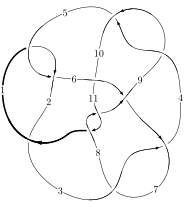
\includegraphics[width=112pt]{../../../GIT/diagram.site/Diagrams/png/364_11a_115.png}\\
\ \ \ A knot diagram\footnotemark}&
\allowdisplaybreaks
\textbf{Linearized knot diagam} \\
\cline{2-2}
 &
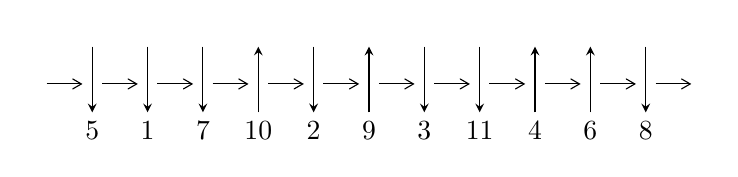
\begin{tikzpicture}[x=20pt, y=17pt]
	% nodes
	\node (C0) at (0, 0) {};
	\node (C1) at (1, 0) {};
	\node (C1U) at (1, +1) {};
	\node (C1D) at (1, -1) {5};

	\node (C2) at (2, 0) {};
	\node (C2U) at (2, +1) {};
	\node (C2D) at (2, -1) {1};

	\node (C3) at (3, 0) {};
	\node (C3U) at (3, +1) {};
	\node (C3D) at (3, -1) {7};

	\node (C4) at (4, 0) {};
	\node (C4U) at (4, +1) {};
	\node (C4D) at (4, -1) {10};

	\node (C5) at (5, 0) {};
	\node (C5U) at (5, +1) {};
	\node (C5D) at (5, -1) {2};

	\node (C6) at (6, 0) {};
	\node (C6U) at (6, +1) {};
	\node (C6D) at (6, -1) {9};

	\node (C7) at (7, 0) {};
	\node (C7U) at (7, +1) {};
	\node (C7D) at (7, -1) {3};

	\node (C8) at (8, 0) {};
	\node (C8U) at (8, +1) {};
	\node (C8D) at (8, -1) {11};

	\node (C9) at (9, 0) {};
	\node (C9U) at (9, +1) {};
	\node (C9D) at (9, -1) {4};

	\node (C10) at (10, 0) {};
	\node (C10U) at (10, +1) {};
	\node (C10D) at (10, -1) {6};

	\node (C11) at (11, 0) {};
	\node (C11U) at (11, +1) {};
	\node (C11D) at (11, -1) {8};
	\node (C12) at (12, 0) {};

	% arrows
	\draw[->,>={angle 60}]
	(C0) edge (C1) (C1) edge (C2) (C2) edge (C3) (C3) edge (C4) (C4) edge (C5) (C5) edge (C6) (C6) edge (C7) (C7) edge (C8) (C8) edge (C9) (C9) edge (C10) (C10) edge (C11) (C11) edge (C12) ;	\draw[->,>=stealth]
	(C1U) edge (C1D) (C2U) edge (C2D) (C3U) edge (C3D) (C4D) edge (C4U) (C5U) edge (C5D) (C6D) edge (C6U) (C7U) edge (C7D) (C8U) edge (C8D) (C9D) edge (C9U) (C10D) edge (C10U) (C11U) edge (C11D) ;
	\end{tikzpicture} \\
\hhline{~~} \\& 
\textbf{Solving Sequence} \\ \cline{2-2} 
 &
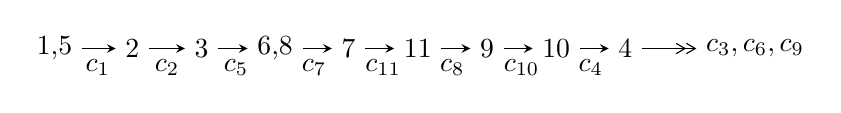
\begin{tikzpicture}[x=25pt, y=7pt]
	% node
	\node (A0) at (-1/8, 0) {1,5};
	\node (A1) at (1, 0) {2};
	\node (A2) at (2, 0) {3};
	\node (A3) at (49/16, 0) {6,8};
	\node (A4) at (33/8, 0) {7};
	\node (A5) at (41/8, 0) {11};
	\node (A6) at (49/8, 0) {9};
	\node (A7) at (57/8, 0) {10};
	\node (A8) at (65/8, 0) {4};
	\node (C1) at (1/2, -1) {$c_{1}$};
	\node (C2) at (3/2, -1) {$c_{2}$};
	\node (C3) at (5/2, -1) {$c_{5}$};
	\node (C4) at (29/8, -1) {$c_{7}$};
	\node (C5) at (37/8, -1) {$c_{11}$};
	\node (C6) at (45/8, -1) {$c_{8}$};
	\node (C7) at (53/8, -1) {$c_{10}$};
	\node (C8) at (61/8, -1) {$c_{4}$};
	\node (A9) at (10, 0) {$c_{3},c_{6},c_{9}$};

	% edge
	\draw[->,>=stealth]	
	(A0) edge (A1) (A1) edge (A2) (A2) edge (A3) (A3) edge (A4) (A4) edge (A5) (A5) edge (A6) (A6) edge (A7) (A7) edge (A8) ;
	\draw[->>,>={angle 60}]	
	(A8) edge (A9);
\end{tikzpicture} \\ 

\end{tabular} \\

\footnotetext{
The image of knot diagram is generated by the software ``\textbf{Draw programme}" developed by Andrew Bartholomew(\url{http://www.layer8.co.uk/maths/draw/index.htm\#Running-draw}), where we modified some parts for our purpose(\url{https://github.com/CATsTAILs/LinksPainter}).
}\phantom \\ \newline 
\centering \textbf{Ideals for irreducible components\footnotemark of $X_{\text{par}}$} 
 
\begin{align*}
I^u_{1}&=\langle 
3.32851\times10^{102} u^{77}-1.61333\times10^{103} u^{76}+\cdots+2.32216\times10^{103} b+2.92650\times10^{103},\\
\phantom{I^u_{1}}&\phantom{= \langle  }-2.22107\times10^{103} u^{77}+8.11330\times10^{103} u^{76}+\cdots+2.32216\times10^{103} a+2.42675\times10^{104},\\
\phantom{I^u_{1}}&\phantom{= \langle  }u^{78}-3 u^{77}+\cdots+10 u+1\rangle \\
I^u_{2}&=\langle 
-2 u^{17}-2 u^{16}+\cdots+b-3,\;-4 u^{17}-5 u^{16}+\cdots+a-3,\;u^{18}+2 u^{17}+\cdots+2 u+1\rangle \\
\\
\end{align*}
\raggedright * 2 irreducible components of $\dim_{\mathbb{C}}=0$, with total 96 representations.\\
\footnotetext{All coefficients of polynomials are rational numbers. But the coefficients are sometimes approximated in decimal forms when there is not enough margin.}
\newpage
\renewcommand{\arraystretch}{1}
\centering \section*{I. $I^u_{1}= \langle 3.33\times10^{102} u^{77}-1.61\times10^{103} u^{76}+\cdots+2.32\times10^{103} b+2.93\times10^{103},\;-2.22\times10^{103} u^{77}+8.11\times10^{103} u^{76}+\cdots+2.32\times10^{103} a+2.43\times10^{104},\;u^{78}-3 u^{77}+\cdots+10 u+1 \rangle$}
\flushleft \textbf{(i) Arc colorings}\\
\begin{tabular}{m{7pt} m{180pt} m{7pt} m{180pt} }
\flushright $a_{1}=$&$\begin{pmatrix}1\\0\end{pmatrix}$ \\
\flushright $a_{5}=$&$\begin{pmatrix}0\\u\end{pmatrix}$ \\
\flushright $a_{2}=$&$\begin{pmatrix}1\\u^2\end{pmatrix}$ \\
\flushright $a_{3}=$&$\begin{pmatrix}- u^2+1\\u^2\end{pmatrix}$ \\
\flushright $a_{6}=$&$\begin{pmatrix}- u\\- u^3+u\end{pmatrix}$ \\
\flushright $a_{8}=$&$\begin{pmatrix}0.956467 u^{77}-3.49386 u^{76}+\cdots+58.2139 u-10.4504\\-0.143337 u^{77}+0.694752 u^{76}+\cdots-11.2798 u-1.26025\end{pmatrix}$ \\
\flushright $a_{7}=$&$\begin{pmatrix}0.623458 u^{77}-2.49883 u^{76}+\cdots+44.5704 u-11.9913\\-0.180850 u^{77}+0.890365 u^{76}+\cdots-11.7000 u-1.33932\end{pmatrix}$ \\
\flushright $a_{11}=$&$\begin{pmatrix}-0.963362 u^{77}+3.15022 u^{76}+\cdots-117.362 u-14.6971\\-0.255022 u^{77}+0.791044 u^{76}+\cdots-5.96319 u+0.0156746\end{pmatrix}$ \\
\flushright $a_{9}=$&$\begin{pmatrix}-0.580789 u^{77}+1.58696 u^{76}+\cdots-51.0047 u-13.6034\\0.323044 u^{77}-1.22096 u^{76}+\cdots-4.39700 u+0.102187\end{pmatrix}$ \\
\flushright $a_{10}=$&$\begin{pmatrix}-1.25538 u^{77}+3.66967 u^{76}+\cdots-115.076 u-14.3275\\-0.0438473 u^{77}+0.659953 u^{76}+\cdots-4.39108 u+0.00274049\end{pmatrix}$ \\
\flushright $a_{4}=$&$\begin{pmatrix}1.66912 u^{77}-5.04900 u^{76}+\cdots+142.099 u+20.3371\\-0.229652 u^{77}+0.323047 u^{76}+\cdots+9.44012 u+0.185234\end{pmatrix}$\\ \flushright $a_{4}=$&$\begin{pmatrix}1.66912 u^{77}-5.04900 u^{76}+\cdots+142.099 u+20.3371\\-0.229652 u^{77}+0.323047 u^{76}+\cdots+9.44012 u+0.185234\end{pmatrix}$\\&\end{tabular}
\flushleft \textbf{(ii) Obstruction class $= -1$}\\~\\
\flushleft \textbf{(iii) Cusp Shapes $= 0.440746 u^{77}+0.132996 u^{76}+\cdots+82.1887 u+8.36358$}\\~\\
\newpage\renewcommand{\arraystretch}{1}
\flushleft \textbf{(iv) u-Polynomials at the component}\newline \\
\begin{tabular}{m{50pt}|m{274pt}}
Crossings & \hspace{64pt}u-Polynomials at each crossing \\
\hline $$\begin{aligned}c_{1},c_{5}\end{aligned}$$&$\begin{aligned}
&u^{78}+3 u^{77}+\cdots-10 u+1
\end{aligned}$\\
\hline $$\begin{aligned}c_{2}\end{aligned}$$&$\begin{aligned}
&u^{78}+27 u^{77}+\cdots-82 u+1
\end{aligned}$\\
\hline $$\begin{aligned}c_{3},c_{7}\end{aligned}$$&$\begin{aligned}
&u^{78}+u^{77}+\cdots+658 u+59
\end{aligned}$\\
\hline $$\begin{aligned}c_{4},c_{9}\end{aligned}$$&$\begin{aligned}
&u^{78}+u^{77}+\cdots-2 u+1
\end{aligned}$\\
\hline $$\begin{aligned}c_{6}\end{aligned}$$&$\begin{aligned}
&u^{78}+10 u^{77}+\cdots+194051 u+23683
\end{aligned}$\\
\hline $$\begin{aligned}c_{8},c_{11}\end{aligned}$$&$\begin{aligned}
&u^{78}-4 u^{77}+\cdots-1235 u+271
\end{aligned}$\\
\hline $$\begin{aligned}c_{10}\end{aligned}$$&$\begin{aligned}
&u^{78}-2 u^{77}+\cdots-34703 u+4663
\end{aligned}$\\
\hline
\end{tabular}\\~\\
\newpage\renewcommand{\arraystretch}{1}
\flushleft \textbf{(v) Riley Polynomials at the component}\newline \\
\begin{tabular}{m{50pt}|m{274pt}}
Crossings & \hspace{64pt}Riley Polynomials at each crossing \\
\hline $$\begin{aligned}c_{1},c_{5}\end{aligned}$$&$\begin{aligned}
&y^{78}-27 y^{77}+\cdots+82 y+1
\end{aligned}$\\
\hline $$\begin{aligned}c_{2}\end{aligned}$$&$\begin{aligned}
&y^{78}+57 y^{77}+\cdots+3662 y+1
\end{aligned}$\\
\hline $$\begin{aligned}c_{3},c_{7}\end{aligned}$$&$\begin{aligned}
&y^{78}+73 y^{77}+\cdots-596276 y+3481
\end{aligned}$\\
\hline $$\begin{aligned}c_{4},c_{9}\end{aligned}$$&$\begin{aligned}
&y^{78}-59 y^{77}+\cdots-128 y+1
\end{aligned}$\\
\hline $$\begin{aligned}c_{6}\end{aligned}$$&$\begin{aligned}
&y^{78}-36 y^{77}+\cdots-17292910371 y+560884489
\end{aligned}$\\
\hline $$\begin{aligned}c_{8},c_{11}\end{aligned}$$&$\begin{aligned}
&y^{78}+60 y^{77}+\cdots-1616823 y+73441
\end{aligned}$\\
\hline $$\begin{aligned}c_{10}\end{aligned}$$&$\begin{aligned}
&y^{78}-32 y^{77}+\cdots-28280283 y+21743569
\end{aligned}$\\
\hline
\end{tabular}\\~\\
\newpage\flushleft \textbf{(vi) Complex Volumes and Cusp Shapes}
$$\begin{array}{c|c|c}  
\text{Solutions to }I^u_{1}& \I (\text{vol} + \sqrt{-1}CS) & \text{Cusp shape}\\
 \hline 
\begin{aligned}
u &= \phantom{-}0.919382 + 0.415096 I \\
a &= -0.319202 - 0.766497 I \\
b &= \phantom{-}0.705973 - 0.119570 I\end{aligned}
 & -1.84172 - 1.54832 I & \phantom{-0.000000 } 0 \\ \hline\begin{aligned}
u &= \phantom{-}0.919382 - 0.415096 I \\
a &= -0.319202 + 0.766497 I \\
b &= \phantom{-}0.705973 + 0.119570 I\end{aligned}
 & -1.84172 + 1.54832 I & \phantom{-0.000000 } 0 \\ \hline\begin{aligned}
u &= \phantom{-}0.651027 + 0.778881 I \\
a &= \phantom{-}0.651319 - 0.808354 I \\
b &= \phantom{-}0.351881 - 0.133943 I\end{aligned}
 & \phantom{-}6.48100 - 3.09388 I & \phantom{-0.000000 } 0 \\ \hline\begin{aligned}
u &= \phantom{-}0.651027 - 0.778881 I \\
a &= \phantom{-}0.651319 + 0.808354 I \\
b &= \phantom{-}0.351881 + 0.133943 I\end{aligned}
 & \phantom{-}6.48100 + 3.09388 I & \phantom{-0.000000 } 0 \\ \hline\begin{aligned}
u &= \phantom{-}0.980487 + 0.091787 I \\
a &= -0.786643 + 0.077505 I \\
b &= -0.441029 - 0.187587 I\end{aligned}
 & -1.67404 - 0.08608 I & \phantom{-0.000000 } 0 \\ \hline\begin{aligned}
u &= \phantom{-}0.980487 - 0.091787 I \\
a &= -0.786643 - 0.077505 I \\
b &= -0.441029 + 0.187587 I\end{aligned}
 & -1.67404 + 0.08608 I & \phantom{-0.000000 } 0 \\ \hline\begin{aligned}
u &= -0.510641 + 0.879678 I \\
a &= -0.07433 + 1.43681 I \\
b &= -0.084266 - 1.336750 I\end{aligned}
 & \phantom{-}7.01017 + 0.55763 I & \phantom{-0.000000 } 0 \\ \hline\begin{aligned}
u &= -0.510641 - 0.879678 I \\
a &= -0.07433 - 1.43681 I \\
b &= -0.084266 + 1.336750 I\end{aligned}
 & \phantom{-}7.01017 - 0.55763 I & \phantom{-0.000000 } 0 \\ \hline\begin{aligned}
u &= -0.683117 + 0.756267 I \\
a &= \phantom{-}0.68410 + 2.40034 I \\
b &= -0.175954 - 1.224060 I\end{aligned}
 & \phantom{-}6.61578 - 3.90393 I & \phantom{-0.000000 } 0 \\ \hline\begin{aligned}
u &= -0.683117 - 0.756267 I \\
a &= \phantom{-}0.68410 - 2.40034 I \\
b &= -0.175954 + 1.224060 I\end{aligned}
 & \phantom{-}6.61578 + 3.90393 I & \phantom{-0.000000 } 0\\
 \hline 
 \end{array}$$\newpage$$\begin{array}{c|c|c}  
\text{Solutions to }I^u_{1}& \I (\text{vol} + \sqrt{-1}CS) & \text{Cusp shape}\\
 \hline 
\begin{aligned}
u &= -0.912558 + 0.348343 I \\
a &= \phantom{-}0.947042 + 0.537303 I \\
b &= \phantom{-}0.787513 - 0.609067 I\end{aligned}
 & -2.10532 + 3.54417 I & \phantom{-0.000000 } 0 \\ \hline\begin{aligned}
u &= -0.912558 - 0.348343 I \\
a &= \phantom{-}0.947042 - 0.537303 I \\
b &= \phantom{-}0.787513 + 0.609067 I\end{aligned}
 & -2.10532 - 3.54417 I & \phantom{-0.000000 } 0 \\ \hline\begin{aligned}
u &= -0.854307 + 0.613428 I \\
a &= -0.502806 - 0.147246 I \\
b &= -0.520280 - 0.175145 I\end{aligned}
 & \phantom{-}2.08259 + 2.42309 I & \phantom{-0.000000 } 0 \\ \hline\begin{aligned}
u &= -0.854307 - 0.613428 I \\
a &= -0.502806 + 0.147246 I \\
b &= -0.520280 + 0.175145 I\end{aligned}
 & \phantom{-}2.08259 - 2.42309 I & \phantom{-0.000000 } 0 \\ \hline\begin{aligned}
u &= \phantom{-}0.785103 + 0.701110 I \\
a &= \phantom{-}0.29828 + 1.88835 I \\
b &= \phantom{-}0.165797 - 1.365190 I\end{aligned}
 & \phantom{-}10.31720 + 0.07253 I & \phantom{-0.000000 } 0 \\ \hline\begin{aligned}
u &= \phantom{-}0.785103 - 0.701110 I \\
a &= \phantom{-}0.29828 - 1.88835 I \\
b &= \phantom{-}0.165797 + 1.365190 I\end{aligned}
 & \phantom{-}10.31720 - 0.07253 I & \phantom{-0.000000 } 0 \\ \hline\begin{aligned}
u &= -1.051310 + 0.134686 I \\
a &= -0.534104 + 0.782333 I \\
b &= -0.661388 - 0.288377 I\end{aligned}
 & \phantom{-}1.42489 + 4.47911 I & \phantom{-0.000000 } 0 \\ \hline\begin{aligned}
u &= -1.051310 - 0.134686 I \\
a &= -0.534104 - 0.782333 I \\
b &= -0.661388 + 0.288377 I\end{aligned}
 & \phantom{-}1.42489 - 4.47911 I & \phantom{-0.000000 } 0 \\ \hline\begin{aligned}
u &= \phantom{-}0.823137 + 0.670951 I \\
a &= -1.04974 + 1.76751 I \\
b &= \phantom{-}0.110492 - 1.219630 I\end{aligned}
 & \phantom{-}2.31988 + 0.18759 I & \phantom{-0.000000 } 0 \\ \hline\begin{aligned}
u &= \phantom{-}0.823137 - 0.670951 I \\
a &= -1.04974 - 1.76751 I \\
b &= \phantom{-}0.110492 + 1.219630 I\end{aligned}
 & \phantom{-}2.31988 - 0.18759 I & \phantom{-0.000000 } 0\\
 \hline 
 \end{array}$$\newpage$$\begin{array}{c|c|c}  
\text{Solutions to }I^u_{1}& \I (\text{vol} + \sqrt{-1}CS) & \text{Cusp shape}\\
 \hline 
\begin{aligned}
u &= -0.625258 + 0.864565 I \\
a &= -0.58964 - 1.50488 I \\
b &= \phantom{-}0.43046 + 1.58093 I\end{aligned}
 & \phantom{-}8.01275 - 4.37942 I & \phantom{-0.000000 } 0 \\ \hline\begin{aligned}
u &= -0.625258 - 0.864565 I \\
a &= -0.58964 + 1.50488 I \\
b &= \phantom{-}0.43046 - 1.58093 I\end{aligned}
 & \phantom{-}8.01275 + 4.37942 I & \phantom{-0.000000 } 0 \\ \hline\begin{aligned}
u &= \phantom{-}0.721996 + 0.787512 I \\
a &= \phantom{-}0.391090 + 0.643123 I \\
b &= -1.205930 + 0.306716 I\end{aligned}
 & \phantom{-}7.57591 + 4.18168 I & \phantom{-0.000000 } 0 \\ \hline\begin{aligned}
u &= \phantom{-}0.721996 - 0.787512 I \\
a &= \phantom{-}0.391090 - 0.643123 I \\
b &= -1.205930 - 0.306716 I\end{aligned}
 & \phantom{-}7.57591 - 4.18168 I & \phantom{-0.000000 } 0 \\ \hline\begin{aligned}
u &= -0.646393 + 0.857994 I \\
a &= -0.57056 - 1.86291 I \\
b &= -0.330634 + 1.210310 I\end{aligned}
 & \phantom{-}6.63045 + 2.08529 I & \phantom{-0.000000 } 0 \\ \hline\begin{aligned}
u &= -0.646393 - 0.857994 I \\
a &= -0.57056 + 1.86291 I \\
b &= -0.330634 - 1.210310 I\end{aligned}
 & \phantom{-}6.63045 - 2.08529 I & \phantom{-0.000000 } 0 \\ \hline\begin{aligned}
u &= \phantom{-}1.091450 + 0.073360 I \\
a &= -0.785955 + 0.496692 I \\
b &= -0.428556 - 1.064990 I\end{aligned}
 & \phantom{-}0.82847 - 3.56102 I & \phantom{-0.000000 } 0 \\ \hline\begin{aligned}
u &= \phantom{-}1.091450 - 0.073360 I \\
a &= -0.785955 - 0.496692 I \\
b &= -0.428556 + 1.064990 I\end{aligned}
 & \phantom{-}0.82847 + 3.56102 I & \phantom{-0.000000 } 0 \\ \hline\begin{aligned}
u &= -0.900766 + 0.062670 I \\
a &= \phantom{-}0.07406 + 1.84676 I \\
b &= -0.241501 + 1.105310 I\end{aligned}
 & \phantom{-}6.20657 - 0.98958 I & \phantom{-}                -6
0.902681 + 0. 10   I\phantom{ +0.000000I} \\ \hline\begin{aligned}
u &= -0.900766 - 0.062670 I \\
a &= \phantom{-}0.07406 - 1.84676 I \\
b &= -0.241501 - 1.105310 I\end{aligned}
 & \phantom{-}6.20657 + 0.98958 I & \phantom{-}                -6
0.902681 + 0. 10   I\phantom{ +0.000000I}\\
 \hline 
 \end{array}$$\newpage$$\begin{array}{c|c|c}  
\text{Solutions to }I^u_{1}& \I (\text{vol} + \sqrt{-1}CS) & \text{Cusp shape}\\
 \hline 
\begin{aligned}
u &= \phantom{-}0.796237 + 0.760422 I \\
a &= \phantom{-}0.738120 - 1.145030 I \\
b &= -0.63396 + 1.61284 I\end{aligned}
 & \phantom{-}11.42440 - 2.49625 I & \phantom{-0.000000 } 0 \\ \hline\begin{aligned}
u &= \phantom{-}0.796237 - 0.760422 I \\
a &= \phantom{-}0.738120 + 1.145030 I \\
b &= -0.63396 - 1.61284 I\end{aligned}
 & \phantom{-}11.42440 + 2.49625 I & \phantom{-0.000000 } 0 \\ \hline\begin{aligned}
u &= -0.867555 + 0.688655 I \\
a &= -0.353143 + 0.969190 I \\
b &= \phantom{-}1.57794 + 0.12915 I\end{aligned}
 & \phantom{-}1.69309 + 2.65199 I & \phantom{-0.000000 } 0 \\ \hline\begin{aligned}
u &= -0.867555 - 0.688655 I \\
a &= -0.353143 - 0.969190 I \\
b &= \phantom{-}1.57794 - 0.12915 I\end{aligned}
 & \phantom{-}1.69309 - 2.65199 I & \phantom{-0.000000 } 0 \\ \hline\begin{aligned}
u &= \phantom{-}0.897871 + 0.675237 I \\
a &= \phantom{-}0.98099 - 2.00046 I \\
b &= \phantom{-}0.327853 + 1.299700 I\end{aligned}
 & \phantom{-}2.08862 - 5.40076 I & \phantom{-0.000000 } 0 \\ \hline\begin{aligned}
u &= \phantom{-}0.897871 - 0.675237 I \\
a &= \phantom{-}0.98099 + 2.00046 I \\
b &= \phantom{-}0.327853 - 1.299700 I\end{aligned}
 & \phantom{-}2.08862 + 5.40076 I & \phantom{-0.000000 } 0 \\ \hline\begin{aligned}
u &= -0.471260 + 0.715322 I \\
a &= \phantom{-}0.367913 + 0.003194 I \\
b &= -0.577762 + 0.019556 I\end{aligned}
 & \phantom{-}3.10549 - 1.21428 I &                  -6
-0.932552 + 0. 10   I\phantom{ +0.000000I} \\ \hline\begin{aligned}
u &= -0.471260 - 0.715322 I \\
a &= \phantom{-}0.367913 - 0.003194 I \\
b &= -0.577762 - 0.019556 I\end{aligned}
 & \phantom{-}3.10549 + 1.21428 I &                  -6
-0.932552 + 0. 10   I\phantom{ +0.000000I} \\ \hline\begin{aligned}
u &= \phantom{-}0.934384 + 0.682083 I \\
a &= \phantom{-}2.19405 - 1.31253 I \\
b &= \phantom{-}0.209204 + 1.238200 I\end{aligned}
 & \phantom{-}9.85296 - 5.39790 I & \phantom{-0.000000 } 0 \\ \hline\begin{aligned}
u &= \phantom{-}0.934384 - 0.682083 I \\
a &= \phantom{-}2.19405 + 1.31253 I \\
b &= \phantom{-}0.209204 - 1.238200 I\end{aligned}
 & \phantom{-}9.85296 + 5.39790 I & \phantom{-0.000000 } 0\\
 \hline 
 \end{array}$$\newpage$$\begin{array}{c|c|c}  
\text{Solutions to }I^u_{1}& \I (\text{vol} + \sqrt{-1}CS) & \text{Cusp shape}\\
 \hline 
\begin{aligned}
u &= -0.806544 + 0.123097 I \\
a &= \phantom{-}0.539789 + 0.141829 I \\
b &= \phantom{-}0.637200 + 0.917242 I\end{aligned}
 & -1.17381 - 1.68388 I & \phantom{-}0.83726 - 6.01771 I \\ \hline\begin{aligned}
u &= -0.806544 - 0.123097 I \\
a &= \phantom{-}0.539789 - 0.141829 I \\
b &= \phantom{-}0.637200 - 0.917242 I\end{aligned}
 & -1.17381 + 1.68388 I & \phantom{-}0.83726 + 6.01771 I \\ \hline\begin{aligned}
u &= \phantom{-}0.940160 + 0.729085 I \\
a &= -1.30654 + 1.57774 I \\
b &= -0.76597 - 1.46965 I\end{aligned}
 & \phantom{-}10.98100 - 3.15371 I & \phantom{-0.000000 } 0 \\ \hline\begin{aligned}
u &= \phantom{-}0.940160 - 0.729085 I \\
a &= -1.30654 - 1.57774 I \\
b &= -0.76597 + 1.46965 I\end{aligned}
 & \phantom{-}10.98100 + 3.15371 I & \phantom{-0.000000 } 0 \\ \hline\begin{aligned}
u &= \phantom{-}0.785464 + 0.142913 I \\
a &= \phantom{-}0.62353 - 1.64939 I \\
b &= \phantom{-}0.831715 + 0.510792 I\end{aligned}
 & -1.32910 - 0.60787 I & -3.50485 - 2.67829 I \\ \hline\begin{aligned}
u &= \phantom{-}0.785464 - 0.142913 I \\
a &= \phantom{-}0.62353 + 1.64939 I \\
b &= \phantom{-}0.831715 - 0.510792 I\end{aligned}
 & -1.32910 + 0.60787 I & -3.50485 + 2.67829 I \\ \hline\begin{aligned}
u &= -1.053060 + 0.586459 I \\
a &= -0.023473 - 0.712350 I \\
b &= -0.590557 + 0.019641 I\end{aligned}
 & \phantom{-}1.39270 + 6.19483 I & \phantom{-0.000000 } 0 \\ \hline\begin{aligned}
u &= -1.053060 - 0.586459 I \\
a &= -0.023473 + 0.712350 I \\
b &= -0.590557 - 0.019641 I\end{aligned}
 & \phantom{-}1.39270 - 6.19483 I & \phantom{-0.000000 } 0 \\ \hline\begin{aligned}
u &= \phantom{-}0.650281 + 1.026430 I \\
a &= \phantom{-}0.39794 - 1.45251 I \\
b &= -0.44162 + 1.48170 I\end{aligned}
 & \phantom{-}13.3117 + 9.8514 I & \phantom{-0.000000 } 0 \\ \hline\begin{aligned}
u &= \phantom{-}0.650281 - 1.026430 I \\
a &= \phantom{-}0.39794 + 1.45251 I \\
b &= -0.44162 - 1.48170 I\end{aligned}
 & \phantom{-}13.3117 - 9.8514 I & \phantom{-0.000000 } 0\\
 \hline 
 \end{array}$$\newpage$$\begin{array}{c|c|c}  
\text{Solutions to }I^u_{1}& \I (\text{vol} + \sqrt{-1}CS) & \text{Cusp shape}\\
 \hline 
\begin{aligned}
u &= -1.003170 + 0.699177 I \\
a &= -1.20363 - 2.06396 I \\
b &= -0.276298 + 1.317430 I\end{aligned}
 & \phantom{-}5.65322 + 9.45248 I & \phantom{-0.000000 } 0 \\ \hline\begin{aligned}
u &= -1.003170 - 0.699177 I \\
a &= -1.20363 + 2.06396 I \\
b &= -0.276298 - 1.317430 I\end{aligned}
 & \phantom{-}5.65322 - 9.45248 I & \phantom{-0.000000 } 0 \\ \hline\begin{aligned}
u &= \phantom{-}0.991949 + 0.723933 I \\
a &= \phantom{-}0.029164 + 0.815832 I \\
b &= -1.324200 - 0.107360 I\end{aligned}
 & \phantom{-}6.75517 - 9.89412 I & \phantom{-0.000000 } 0 \\ \hline\begin{aligned}
u &= \phantom{-}0.991949 - 0.723933 I \\
a &= \phantom{-}0.029164 - 0.815832 I \\
b &= -1.324200 + 0.107360 I\end{aligned}
 & \phantom{-}6.75517 + 9.89412 I & \phantom{-0.000000 } 0 \\ \hline\begin{aligned}
u &= \phantom{-}1.224710 + 0.112853 I \\
a &= \phantom{-}0.237600 + 0.305151 I \\
b &= \phantom{-}0.268395 + 1.179100 I\end{aligned}
 & \phantom{-}1.03395 - 3.16868 I & \phantom{-0.000000 } 0 \\ \hline\begin{aligned}
u &= \phantom{-}1.224710 - 0.112853 I \\
a &= \phantom{-}0.237600 - 0.305151 I \\
b &= \phantom{-}0.268395 - 1.179100 I\end{aligned}
 & \phantom{-}1.03395 + 3.16868 I & \phantom{-0.000000 } 0 \\ \hline\begin{aligned}
u &= \phantom{-}1.025600 + 0.727427 I \\
a &= \phantom{-}0.186084 + 0.163814 I \\
b &= \phantom{-}0.616269 - 0.163910 I\end{aligned}
 & \phantom{-}5.36964 - 2.62564 I & \phantom{-0.000000 } 0 \\ \hline\begin{aligned}
u &= \phantom{-}1.025600 - 0.727427 I \\
a &= \phantom{-}0.186084 - 0.163814 I \\
b &= \phantom{-}0.616269 + 0.163910 I\end{aligned}
 & \phantom{-}5.36964 + 2.62564 I & \phantom{-0.000000 } 0 \\ \hline\begin{aligned}
u &= -1.058580 + 0.726505 I \\
a &= \phantom{-}1.27853 + 1.47897 I \\
b &= \phantom{-}0.60139 - 1.55104 I\end{aligned}
 & \phantom{-}6.70371 + 10.29660 I & \phantom{-0.000000 } 0 \\ \hline\begin{aligned}
u &= -1.058580 - 0.726505 I \\
a &= \phantom{-}1.27853 - 1.47897 I \\
b &= \phantom{-}0.60139 + 1.55104 I\end{aligned}
 & \phantom{-}6.70371 - 10.29660 I & \phantom{-0.000000 } 0\\
 \hline 
 \end{array}$$\newpage$$\begin{array}{c|c|c}  
\text{Solutions to }I^u_{1}& \I (\text{vol} + \sqrt{-1}CS) & \text{Cusp shape}\\
 \hline 
\begin{aligned}
u &= -1.040720 + 0.774309 I \\
a &= \phantom{-}0.70860 + 1.25362 I \\
b &= -0.097731 - 1.271840 I\end{aligned}
 & \phantom{-}5.46363 + 3.99334 I & \phantom{-0.000000 } 0 \\ \hline\begin{aligned}
u &= -1.040720 - 0.774309 I \\
a &= \phantom{-}0.70860 - 1.25362 I \\
b &= -0.097731 + 1.271840 I\end{aligned}
 & \phantom{-}5.46363 - 3.99334 I & \phantom{-0.000000 } 0 \\ \hline\begin{aligned}
u &= -1.098500 + 0.730187 I \\
a &= -1.24857 - 1.08059 I \\
b &= -0.254548 + 1.221860 I\end{aligned}
 & \phantom{-}5.29888 + 5.39356 I & \phantom{-0.000000 } 0 \\ \hline\begin{aligned}
u &= -1.098500 - 0.730187 I \\
a &= -1.24857 + 1.08059 I \\
b &= -0.254548 - 1.221860 I\end{aligned}
 & \phantom{-}5.29888 - 5.39356 I & \phantom{-0.000000 } 0 \\ \hline\begin{aligned}
u &= \phantom{-}1.115900 + 0.788410 I \\
a &= -1.18485 + 1.48176 I \\
b &= -0.55541 - 1.48099 I\end{aligned}
 & \phantom{-}11.8295 - 16.4283 I & \phantom{-0.000000 } 0 \\ \hline\begin{aligned}
u &= \phantom{-}1.115900 - 0.788410 I \\
a &= -1.18485 - 1.48176 I \\
b &= -0.55541 + 1.48099 I\end{aligned}
 & \phantom{-}11.8295 + 16.4283 I & \phantom{-0.000000 } 0 \\ \hline\begin{aligned}
u &= \phantom{-}0.45896 + 1.35957 I \\
a &= -0.065261 + 1.254430 I \\
b &= \phantom{-}0.046387 - 1.281840 I\end{aligned}
 & \phantom{-}10.84600 - 2.03461 I & \phantom{-0.000000 } 0 \\ \hline\begin{aligned}
u &= \phantom{-}0.45896 - 1.35957 I \\
a &= -0.065261 - 1.254430 I \\
b &= \phantom{-}0.046387 + 1.281840 I\end{aligned}
 & \phantom{-}10.84600 + 2.03461 I & \phantom{-0.000000 } 0 \\ \hline\begin{aligned}
u &= -1.43030 + 0.30968 I \\
a &= -0.462230 - 0.259484 I \\
b &= -0.251800 + 1.189590 I\end{aligned}
 & \phantom{-}4.19571 + 7.76962 I & \phantom{-0.000000 } 0 \\ \hline\begin{aligned}
u &= -1.43030 - 0.30968 I \\
a &= -0.462230 + 0.259484 I \\
b &= -0.251800 - 1.189590 I\end{aligned}
 & \phantom{-}4.19571 - 7.76962 I & \phantom{-0.000000 } 0\\
 \hline 
 \end{array}$$\newpage$$\begin{array}{c|c|c}  
\text{Solutions to }I^u_{1}& \I (\text{vol} + \sqrt{-1}CS) & \text{Cusp shape}\\
 \hline 
\begin{aligned}
u &= -0.489302 + 0.114434 I \\
a &= -1.24057 + 1.69081 I \\
b &= -0.11108 - 1.50372 I\end{aligned}
 & \phantom{-}7.78823 + 1.62906 I & -3.05008 - 4.47531 I \\ \hline\begin{aligned}
u &= -0.489302 - 0.114434 I \\
a &= -1.24057 - 1.69081 I \\
b &= -0.11108 + 1.50372 I\end{aligned}
 & \phantom{-}7.78823 - 1.62906 I & -3.05008 + 4.47531 I \\ \hline\begin{aligned}
u &= \phantom{-}1.24794 + 0.95730 I \\
a &= \phantom{-}0.717195 - 1.121420 I \\
b &= \phantom{-}0.280618 + 1.201350 I\end{aligned}
 & \phantom{-}8.51017 - 5.96874 I & \phantom{-0.000000 } 0 \\ \hline\begin{aligned}
u &= \phantom{-}1.24794 - 0.95730 I \\
a &= \phantom{-}0.717195 + 1.121420 I \\
b &= \phantom{-}0.280618 - 1.201350 I\end{aligned}
 & \phantom{-}8.51017 + 5.96874 I & \phantom{-0.000000 } 0 \\ \hline\begin{aligned}
u &= \phantom{-}0.013339 + 0.320104 I \\
a &= -1.39879 - 0.45191 I \\
b &= \phantom{-}0.373310 + 0.454562 I\end{aligned}
 & -0.078062 - 1.100560 I & -1.42175 + 6.23894 I \\ \hline\begin{aligned}
u &= \phantom{-}0.013339 - 0.320104 I \\
a &= -1.39879 + 0.45191 I \\
b &= \phantom{-}0.373310 - 0.454562 I\end{aligned}
 & -0.078062 + 1.100560 I & -1.42175 - 6.23894 I \\ \hline\begin{aligned}
u &= -0.0520369 + 0.1011840 I \\
a &= -15.3453 + 3.5674 I \\
b &= -0.351925 - 0.721276 I\end{aligned}
 & \phantom{-}5.14575 - 3.44483 I & \phantom{-}3.90868 + 8.31277 I \\ \hline\begin{aligned}
u &= -0.0520369 - 0.1011840 I \\
a &= -15.3453 - 3.5674 I \\
b &= -0.351925 + 0.721276 I\end{aligned}
 & \phantom{-}5.14575 + 3.44483 I & \phantom{-}3.90868 - 8.31277 I\\
 \hline 
 \end{array}$$\newpage\newpage\renewcommand{\arraystretch}{1}
\centering \section*{II. $I^u_{2}= \langle -2 u^{17}-2 u^{16}+\cdots+b-3,\;-4 u^{17}-5 u^{16}+\cdots+a-3,\;u^{18}+2 u^{17}+\cdots+2 u+1 \rangle$}
\flushleft \textbf{(i) Arc colorings}\\
\begin{tabular}{m{7pt} m{180pt} m{7pt} m{180pt} }
\flushright $a_{1}=$&$\begin{pmatrix}1\\0\end{pmatrix}$ \\
\flushright $a_{5}=$&$\begin{pmatrix}0\\u\end{pmatrix}$ \\
\flushright $a_{2}=$&$\begin{pmatrix}1\\u^2\end{pmatrix}$ \\
\flushright $a_{3}=$&$\begin{pmatrix}- u^2+1\\u^2\end{pmatrix}$ \\
\flushright $a_{6}=$&$\begin{pmatrix}- u\\- u^3+u\end{pmatrix}$ \\
\flushright $a_{8}=$&$\begin{pmatrix}4 u^{17}+5 u^{16}+\cdots+3 u+3\\2 u^{17}+2 u^{16}+\cdots+5 u+3\end{pmatrix}$ \\
\flushright $a_{7}=$&$\begin{pmatrix}3 u^{17}+3 u^{16}+\cdots+3 u+1\\2 u^{17}+2 u^{16}+\cdots+6 u+3\end{pmatrix}$ \\
\flushright $a_{11}=$&$\begin{pmatrix}3 u^{17}+6 u^{16}+\cdots+4 u+8\\-2 u^{17}-4 u^{16}+\cdots+9 u^2-1\end{pmatrix}$ \\
\flushright $a_{9}=$&$\begin{pmatrix}u^{17}-3 u^{15}+\cdots+9 u^2-4\\- u^{16}-3 u^{15}+\cdots+4 u+3\end{pmatrix}$ \\
\flushright $a_{10}=$&$\begin{pmatrix}4 u^{17}+7 u^{16}+\cdots+3 u+6\\- u^{17}-2 u^{16}+\cdots+2 u+2\end{pmatrix}$ \\
\flushright $a_{4}=$&$\begin{pmatrix}2 u^{17}+4 u^{16}+\cdots-13 u^2+5\\- u^{17}+4 u^{15}+\cdots- u+2\end{pmatrix}$\\ \flushright $a_{4}=$&$\begin{pmatrix}2 u^{17}+4 u^{16}+\cdots-13 u^2+5\\- u^{17}+4 u^{15}+\cdots- u+2\end{pmatrix}$\\&\end{tabular}
\flushleft \textbf{(ii) Obstruction class $= 1$}\\~\\
\flushleft \textbf{(iii) Cusp Shapes $= 4 u^{17}+12 u^{16}+7 u^{15}-17 u^{14}-12 u^{13}+41 u^{12}+54 u^{11}-33 u^{10}-85 u^9+12 u^8+97 u^7- u^6-90 u^5-6 u^4+70 u^3+18 u^2-28 u-16$}\\~\\
\newpage\renewcommand{\arraystretch}{1}
\flushleft \textbf{(iv) u-Polynomials at the component}\newline \\
\begin{tabular}{m{50pt}|m{274pt}}
Crossings & \hspace{64pt}u-Polynomials at each crossing \\
\hline $$\begin{aligned}c_{1}\end{aligned}$$&$\begin{aligned}
&u^{18}+2 u^{17}+\cdots+2 u+1
\end{aligned}$\\
\hline $$\begin{aligned}c_{2}\end{aligned}$$&$\begin{aligned}
&u^{18}+8 u^{17}+\cdots+8 u+1
\end{aligned}$\\
\hline $$\begin{aligned}c_{3}\end{aligned}$$&$\begin{aligned}
&u^{18}+10 u^{16}+\cdots-6 u+1
\end{aligned}$\\
\hline $$\begin{aligned}c_{4}\end{aligned}$$&$\begin{aligned}
&u^{18}-6 u^{16}+\cdots+9 u^2+1
\end{aligned}$\\
\hline $$\begin{aligned}c_{5}\end{aligned}$$&$\begin{aligned}
&u^{18}-2 u^{17}+\cdots-2 u+1
\end{aligned}$\\
\hline $$\begin{aligned}c_{6}\end{aligned}$$&$\begin{aligned}
&u^{18}+3 u^{17}+\cdots+7 u+1
\end{aligned}$\\
\hline $$\begin{aligned}c_{7}\end{aligned}$$&$\begin{aligned}
&u^{18}+10 u^{16}+\cdots+6 u+1
\end{aligned}$\\
\hline $$\begin{aligned}c_{8}\end{aligned}$$&$\begin{aligned}
&u^{18}-3 u^{17}+\cdots-3 u+1
\end{aligned}$\\
\hline $$\begin{aligned}c_{9}\end{aligned}$$&$\begin{aligned}
&u^{18}-6 u^{16}+\cdots+9 u^2+1
\end{aligned}$\\
\hline $$\begin{aligned}c_{10}\end{aligned}$$&$\begin{aligned}
&u^{18}+u^{17}+\cdots+u+1
\end{aligned}$\\
\hline $$\begin{aligned}c_{11}\end{aligned}$$&$\begin{aligned}
&u^{18}+3 u^{17}+\cdots+3 u+1
\end{aligned}$\\
\hline
\end{tabular}\\~\\
\newpage\renewcommand{\arraystretch}{1}
\flushleft \textbf{(v) Riley Polynomials at the component}\newline \\
\begin{tabular}{m{50pt}|m{274pt}}
Crossings & \hspace{64pt}Riley Polynomials at each crossing \\
\hline $$\begin{aligned}c_{1},c_{5}\end{aligned}$$&$\begin{aligned}
&y^{18}-8 y^{17}+\cdots-8 y+1
\end{aligned}$\\
\hline $$\begin{aligned}c_{2}\end{aligned}$$&$\begin{aligned}
&y^{18}+12 y^{17}+\cdots+8 y+1
\end{aligned}$\\
\hline $$\begin{aligned}c_{3},c_{7}\end{aligned}$$&$\begin{aligned}
&y^{18}+20 y^{17}+\cdots+2 y+1
\end{aligned}$\\
\hline $$\begin{aligned}c_{4},c_{9}\end{aligned}$$&$\begin{aligned}
&y^{18}-12 y^{17}+\cdots+18 y+1
\end{aligned}$\\
\hline $$\begin{aligned}c_{6}\end{aligned}$$&$\begin{aligned}
&y^{18}-5 y^{17}+\cdots-17 y+1
\end{aligned}$\\
\hline $$\begin{aligned}c_{8},c_{11}\end{aligned}$$&$\begin{aligned}
&y^{18}+11 y^{17}+\cdots+7 y+1
\end{aligned}$\\
\hline $$\begin{aligned}c_{10}\end{aligned}$$&$\begin{aligned}
&y^{18}-5 y^{17}+\cdots-9 y+1
\end{aligned}$\\
\hline
\end{tabular}\\~\\
\newpage\flushleft \textbf{(vi) Complex Volumes and Cusp Shapes}
$$\begin{array}{c|c|c}  
\text{Solutions to }I^u_{2}& \I (\text{vol} + \sqrt{-1}CS) & \text{Cusp shape}\\
 \hline 
\begin{aligned}
u &= \phantom{-}0.600980 + 0.789755 I \\
a &= -0.005827 + 0.968886 I \\
b &= \phantom{-}0.244466 - 1.282710 I\end{aligned}
 & \phantom{-}9.11732 - 1.68939 I & \phantom{-}4.72142 + 2.78192 I \\ \hline\begin{aligned}
u &= \phantom{-}0.600980 - 0.789755 I \\
a &= -0.005827 - 0.968886 I \\
b &= \phantom{-}0.244466 + 1.282710 I\end{aligned}
 & \phantom{-}9.11732 + 1.68939 I & \phantom{-}4.72142 - 2.78192 I \\ \hline\begin{aligned}
u &= \phantom{-}0.882213 + 0.342814 I \\
a &= \phantom{-}0.473394 + 1.217710 I \\
b &= -0.686177 - 0.146117 I\end{aligned}
 & -1.03138 - 1.46977 I & \phantom{-}0.74998 + 4.28225 I \\ \hline\begin{aligned}
u &= \phantom{-}0.882213 - 0.342814 I \\
a &= \phantom{-}0.473394 - 1.217710 I \\
b &= -0.686177 + 0.146117 I\end{aligned}
 & -1.03138 + 1.46977 I & \phantom{-}0.74998 - 4.28225 I \\ \hline\begin{aligned}
u &= -0.867359 + 0.630592 I \\
a &= -0.069787 - 0.673710 I \\
b &= -1.169260 - 0.096853 I\end{aligned}
 & \phantom{-}0.76282 + 2.46662 I & -3.87434 - 2.61953 I \\ \hline\begin{aligned}
u &= -0.867359 - 0.630592 I \\
a &= -0.069787 + 0.673710 I \\
b &= -1.169260 + 0.096853 I\end{aligned}
 & \phantom{-}0.76282 - 2.46662 I & -3.87434 + 2.61953 I \\ \hline\begin{aligned}
u &= \phantom{-}0.878300 + 0.073533 I \\
a &= -0.610367 + 0.158854 I \\
b &= -0.545461 - 0.836793 I\end{aligned}
 & -1.39353 - 2.18547 I & -5.73139 + 7.17501 I \\ \hline\begin{aligned}
u &= \phantom{-}0.878300 - 0.073533 I \\
a &= -0.610367 - 0.158854 I \\
b &= -0.545461 + 0.836793 I\end{aligned}
 & -1.39353 + 2.18547 I & -5.73139 - 7.17501 I \\ \hline\begin{aligned}
u &= -1.141810 + 0.444651 I \\
a &= -0.300052 + 0.568408 I \\
b &= \phantom{-}0.123838 - 0.630055 I\end{aligned}
 & \phantom{-}2.86239 + 5.92628 I & \phantom{-}1.35739 - 5.49734 I \\ \hline\begin{aligned}
u &= -1.141810 - 0.444651 I \\
a &= -0.300052 - 0.568408 I \\
b &= \phantom{-}0.123838 + 0.630055 I\end{aligned}
 & \phantom{-}2.86239 - 5.92628 I & \phantom{-}1.35739 + 5.49734 I\\
 \hline 
 \end{array}$$\newpage$$\begin{array}{c|c|c}  
\text{Solutions to }I^u_{2}& \I (\text{vol} + \sqrt{-1}CS) & \text{Cusp shape}\\
 \hline 
\begin{aligned}
u &= \phantom{-}0.963245 + 0.833701 I \\
a &= \phantom{-}1.17457 - 1.26015 I \\
b &= \phantom{-}0.342226 + 1.036720 I\end{aligned}
 & \phantom{-}8.06866 - 4.51985 I & \phantom{-}3.88251 + 3.07468 I \\ \hline\begin{aligned}
u &= \phantom{-}0.963245 - 0.833701 I \\
a &= \phantom{-}1.17457 + 1.26015 I \\
b &= \phantom{-}0.342226 - 1.036720 I\end{aligned}
 & \phantom{-}8.06866 + 4.51985 I & \phantom{-}3.88251 - 3.07468 I \\ \hline\begin{aligned}
u &= -0.667472 + 0.285364 I \\
a &= -1.11513 + 2.54893 I \\
b &= \phantom{-}0.325026 + 0.632338 I\end{aligned}
 & \phantom{-}4.80242 - 2.81861 I & -1.84387 - 0.52056 I \\ \hline\begin{aligned}
u &= -0.667472 - 0.285364 I \\
a &= -1.11513 - 2.54893 I \\
b &= \phantom{-}0.325026 - 0.632338 I\end{aligned}
 & \phantom{-}4.80242 + 2.81861 I & -1.84387 + 0.52056 I \\ \hline\begin{aligned}
u &= -0.482522 + 0.541462 I \\
a &= -0.41220 + 2.30716 I \\
b &= \phantom{-}0.04482 - 1.43171 I\end{aligned}
 & \phantom{-}8.48319 - 0.98511 I & \phantom{-}5.24254 - 0.71087 I \\ \hline\begin{aligned}
u &= -0.482522 - 0.541462 I \\
a &= -0.41220 - 2.30716 I \\
b &= \phantom{-}0.04482 + 1.43171 I\end{aligned}
 & \phantom{-}8.48319 + 0.98511 I & \phantom{-}5.24254 + 0.71087 I \\ \hline\begin{aligned}
u &= -1.165580 + 0.721113 I \\
a &= -1.13459 - 1.06778 I \\
b &= -0.179481 + 1.292250 I\end{aligned}
 & \phantom{-}6.16158 + 6.28946 I & \phantom{-}3.99576 - 6.33325 I \\ \hline\begin{aligned}
u &= -1.165580 - 0.721113 I \\
a &= -1.13459 + 1.06778 I \\
b &= -0.179481 - 1.292250 I\end{aligned}
 & \phantom{-}6.16158 - 6.28946 I & \phantom{-}3.99576 + 6.33325 I\\
 \hline 
 \end{array}$$\newpage
\newpage\renewcommand{\arraystretch}{1}
\centering \section*{ III. u-Polynomials}
\begin{tabular}{m{50pt}|m{274pt}}
Crossings & \hspace{64pt}u-Polynomials at each crossing \\
\hline $$\begin{aligned}c_{1}\end{aligned}$$&$\begin{aligned}
&(u^{18}+2 u^{17}+\cdots+2 u+1)(u^{78}+3 u^{77}+\cdots-10 u+1)
\end{aligned}$\\
\hline $$\begin{aligned}c_{2}\end{aligned}$$&$\begin{aligned}
&(u^{18}+8 u^{17}+\cdots+8 u+1)(u^{78}+27 u^{77}+\cdots-82 u+1)
\end{aligned}$\\
\hline $$\begin{aligned}c_{3}\end{aligned}$$&$\begin{aligned}
&(u^{18}+10 u^{16}+\cdots-6 u+1)(u^{78}+u^{77}+\cdots+658 u+59)
\end{aligned}$\\
\hline $$\begin{aligned}c_{4}\end{aligned}$$&$\begin{aligned}
&(u^{18}-6 u^{16}+\cdots+9 u^2+1)(u^{78}+u^{77}+\cdots-2 u+1)
\end{aligned}$\\
\hline $$\begin{aligned}c_{5}\end{aligned}$$&$\begin{aligned}
&(u^{18}-2 u^{17}+\cdots-2 u+1)(u^{78}+3 u^{77}+\cdots-10 u+1)
\end{aligned}$\\
\hline $$\begin{aligned}c_{6}\end{aligned}$$&$\begin{aligned}
&(u^{18}+3 u^{17}+\cdots+7 u+1)(u^{78}+10 u^{77}+\cdots+194051 u+23683)
\end{aligned}$\\
\hline $$\begin{aligned}c_{7}\end{aligned}$$&$\begin{aligned}
&(u^{18}+10 u^{16}+\cdots+6 u+1)(u^{78}+u^{77}+\cdots+658 u+59)
\end{aligned}$\\
\hline $$\begin{aligned}c_{8}\end{aligned}$$&$\begin{aligned}
&(u^{18}-3 u^{17}+\cdots-3 u+1)(u^{78}-4 u^{77}+\cdots-1235 u+271)
\end{aligned}$\\
\hline $$\begin{aligned}c_{9}\end{aligned}$$&$\begin{aligned}
&(u^{18}-6 u^{16}+\cdots+9 u^2+1)(u^{78}+u^{77}+\cdots-2 u+1)
\end{aligned}$\\
\hline $$\begin{aligned}c_{10}\end{aligned}$$&$\begin{aligned}
&(u^{18}+u^{17}+\cdots+u+1)(u^{78}-2 u^{77}+\cdots-34703 u+4663)
\end{aligned}$\\
\hline $$\begin{aligned}c_{11}\end{aligned}$$&$\begin{aligned}
&(u^{18}+3 u^{17}+\cdots+3 u+1)(u^{78}-4 u^{77}+\cdots-1235 u+271)
\end{aligned}$\\
\hline
\end{tabular}\newpage\renewcommand{\arraystretch}{1}
\centering \section*{ IV. Riley Polynomials}
\begin{tabular}{m{50pt}|m{274pt}}
Crossings & \hspace{64pt}Riley Polynomials at each crossing \\
\hline $$\begin{aligned}c_{1},c_{5}\end{aligned}$$&$\begin{aligned}
&(y^{18}-8 y^{17}+\cdots-8 y+1)(y^{78}-27 y^{77}+\cdots+82 y+1)
\end{aligned}$\\
\hline $$\begin{aligned}c_{2}\end{aligned}$$&$\begin{aligned}
&(y^{18}+12 y^{17}+\cdots+8 y+1)(y^{78}+57 y^{77}+\cdots+3662 y+1)
\end{aligned}$\\
\hline $$\begin{aligned}c_{3},c_{7}\end{aligned}$$&$\begin{aligned}
&(y^{18}+20 y^{17}+\cdots+2 y+1)(y^{78}+73 y^{77}+\cdots-596276 y+3481)
\end{aligned}$\\
\hline $$\begin{aligned}c_{4},c_{9}\end{aligned}$$&$\begin{aligned}
&(y^{18}-12 y^{17}+\cdots+18 y+1)(y^{78}-59 y^{77}+\cdots-128 y+1)
\end{aligned}$\\
\hline $$\begin{aligned}c_{6}\end{aligned}$$&$\begin{aligned}
&(y^{18}-5 y^{17}+\cdots-17 y+1)\\
&\cdot(y^{78}-36 y^{77}+\cdots-17292910371 y+560884489)
\end{aligned}$\\
\hline $$\begin{aligned}c_{8},c_{11}\end{aligned}$$&$\begin{aligned}
&(y^{18}+11 y^{17}+\cdots+7 y+1)(y^{78}+60 y^{77}+\cdots-1616823 y+73441)
\end{aligned}$\\
\hline $$\begin{aligned}c_{10}\end{aligned}$$&$\begin{aligned}
&(y^{18}-5 y^{17}+\cdots-9 y+1)\\
&\cdot(y^{78}-32 y^{77}+\cdots-28280283 y+21743569)
\end{aligned}$\\
\hline
\end{tabular}
\vskip 2pc
\end{document}